\chapter{Auxiliary Programs}%
\label{cha:Auxiliary_Programs}
\section{Using Ydiff to check results}
\label{sec:Ydiff to check results}

Delivered with Infinity Cinelerra and in the Cinelerra path, there is a file \ {}``ydiff.C''. \ This program compares the output from 2 files to see the differences . \ Do: cd cin\_path and key in ``make ydiff''. 
\medskip

You can now use this to check the quality differences of various outputs. \ For example, in this same directory key in:
\hspace{2em}./ydiff /tmp/yourfile.mp4 /tmp/yourfile.mp4 
\medskip

Since you are comparing a file to itself, you will see a clean looking white window in the left-hand corner and columns 2,3,4 will be all zeros. \ Run this same command with a 3rd spacing parameter of {}-1 as shown below, and you will see artifacts of comparing 2 files starting in a different position.
\medskip

\hspace{2em}./ydiff /tmp/yourfile.mp4 /tmp/yourfile.mp4 -1
\medskip

Now render yourfile using different quality levels and run ydiff to compare the 2 results. \ You will see only noise difference which accounts for the quality level. \ Columns 2,3,4 might no longer be exactly zero but will represent only noise differences. \ The ydiff output is debug data with lines that show frame size in bytes, sum of error, and sum of absolute value of error. \ The frames size is sort of useless, the sum of error shows frame gray point drift and the abs error is the total linear color error between the images. \ At the very end is the total gray point drift and total absolute error on the last line.

{					% uses braces to localize caption alignment changes.
\begin{figure}
	\captionsetup{justification=raggedright,singlelinecheck=false}
	
\includegraphics[width=0.4\linewidth]{ydiff_same.png}
	\caption{Exact match}
	\vspace{-9cm}
 	\hspace{0.4\linewidth}
	\captionsetup{justification=raggedleft,singlelinecheck=false}
	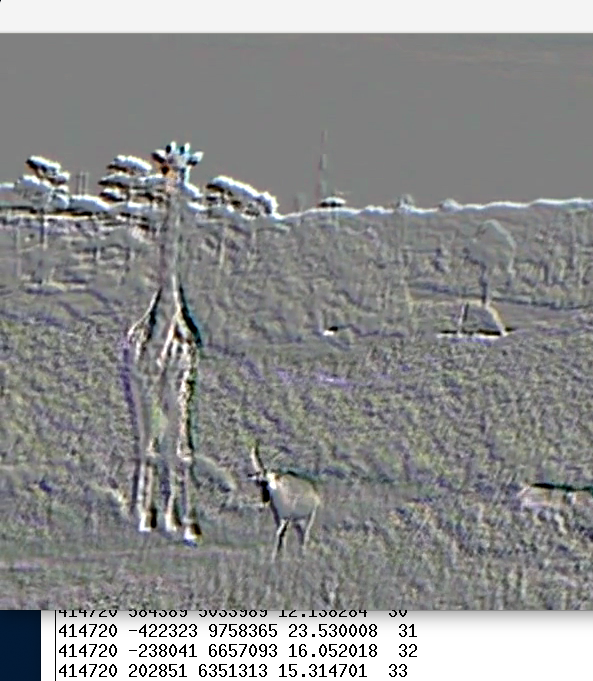
\includegraphics[width=0.4\linewidth]{ydiff_change.png}
	\caption{{\textquotedbl}giraffe{\textquotedbl} artifacts on 2 files spaced differently}
\end{figure}
}
\clearpage

\section{Image Sequence Creation}
\label{sec:Image Sequence Creation}
Example script to create a jpeglist sequence file is next:
\medskip

\begin{lstlisting}[numbers=none]
#!/bin/bash
out="$1"
dir=`dirname "$out"`
shift
geom=`jpegtopnm "$1" | head -2 | tail -1`
w=`(set - $geom; echo $1)`
h=`(set - $geom; echo $2)`
exec > $out
echo "JPEGLIST"
echo "# First line is always JPEGLIST"
echo "# Frame rate:"
echo "29.970030"
echo "# Width:"
echo "$w"
echo "# Height:"
echo "$h"
echo "# List of image files follows"
while [ $# -gt 0 ]; do
if [ x`dirname "$1"` = x"$dir" ]; then f=./`basename "$1"`; else f="$1"; fi
echo "$f"
shift
done
\end{lstlisting}
\medskip

Example usage of this script follows:
\medskip

\ \ \ \ \ jpeglist.sh outfile infiles*.jpg
\medskip

\section{Webm / Vp9 Usage and Example File (credit Frederic Roenitz)}
\label{sec:Webm / Vp9 Usage and Example File}

There are some common VP9 rendering options files that support creation of video for YouTube, Dailymotion, and other online video services. \ Webm / VP9 \ is a media file format which is free to use under the BSD license and is open-source; thus there are no licensing issues to be concerned about. \ The Webm container is based on Matroska for video and Opus for audio.
\medskip

Youtube easy startup steps are documented in the previous section, A.2. \ These same steps have been verified to work for creating Dailymotion videos -- however, the created files must be renamed before uploading to change the youtube extension to webm instead for Dailymotion.

{}- - - - - - - - - - - - - - - - - - - - - - - - - - - - - - - - - - - - - - - - - - - -
\medskip

Below is one of the VP9 rendering options file with documentation for specifics:
\medskip

webm libvpx-vp9
\medskip

\# 20171114-2203
\# from https://developers.google.com/media/vp9/settings/vod/
\# 1280x720 (24, 25 or 30 frames per second)
\#
\#
\# Bitrate (bit rate)
\#

\# VP9 supports several different bitrate modes:
\# mode 
\# Constant Quantizer (Q) \ \ Allows you to specify a fixed quantizer value; bitrate will vary
\# Constrained Quality (CQ) Allows you to set a maximum quality level. Quality may vary within bitrate parameters
\# Variable Bitrate (VBR) \ \ Balances quality and bitrate over time within constraints on bitrate
\# Constant Bitrate (CBR) \ \ Attempts to keep the bitrate fairly constant while quality varies

\#
\# CQ mode is recommended for file-based video (as opposed to live
\# streaming). The following FFMpeg command-line parameters are used
\# for CQ mode:
\#
\# FFMpeg 
\# -b:v {\textless}arg{\textgreater} \ \ \ \ \ Sets target bitrate (e.g. 500k)
\# -minrate {\textless}arg{\textgreater} Sets minimum bitrate.
\# -maxrate {\textless}arg{\textgreater} Sets maximum bitrate.
\# -crf {\textless}arg{\textgreater} Sets maximum quality level. Valid values are 0-63, lower numbers are higher quality.
\#
\# Note: Bitrate is specified in kbps, or kilobits per second. In video
\# compression a kilobit is generally assumed to be 1000 bits (not
\# 1024).
\#
\# Note: Other codecs in FFMpeg accept the -crf parameter but may
\# interpret the value differently. If you are using -crf with other
\# codecs you will likely use different values for VP9.

bitrate=1024k

minrate=512k

maxrate=1485k

crf=32
\medskip

\# Tiling splits the video into rectangular regions, which allows
\# multi-threading for encoding and decoding. The number of tiles is
\# always a power of two. 0=1 tile, 1=2, 2=4, 3=8, 4=16, 5=32.
tile-columns=2
\medskip

\# modified from https://trac.ffmpeg.org/wiki/EncodingForStreamingSites
\# To use a 2 second GOP (Group of Pictures), simply multiply your output
\# frame rate * 2. For example, if your input is -framerate 30, then use
\# -g 60.
g=240
\medskip

\# number of threads to use during encoding.
threads=8
\medskip

\# May be set to good, best, or realtime
quality=good
\medskip

\# This parameter has different meanings depending upon whether quality
\# is set to good or realtime. Speed settings 0-4 apply for VoD in good
\# and best, with 0 being the highest quality and 4 being the
\# lowest. Realtime valid values are 5-8; lower numbers mean higher
\# quality
\medskip

speed=4

\section{Details about .bcast5 Files}
\label{sec:Details about .bcast5 Files}
\medskip

The following extensions of files in Cinelerra's .bcast5 directory are explained below.

% Labeling requires a parameter with the longest word of the labels.
\begin{labeling}{ladspa\_plugins{\dots}}
	\item [.dat] represent saved ``data'' for perpertual sessions and color palettes; maybe others
	\item [.idx] original ``index'' files that were created for loaded video to speed up seeking
	\item [.mkr] ffmpeg specific ``marker'' index file that is created for each video to aid seeks
	\item [.rc] rc stands for ``run commands'' so basically represents a script
	\item [.toc] toc is ``table of contents'' file for MPEG video files (a type of index)
	\item [Cinelerra\_plugins] a list of the currently loaded plugins available in your Cinelerra session
	\item [Cinelerra\_rc] the user's preferences and settings are saved in this file to be used on startup
	\item [ladspa\_plugins{\dots}] ist of currently loaded ladspa plugins for each version of Cinelerra being used
	\item [layout\#...\_rc] user-defined window layout setup with the layout name as part of the file name
	\item [.xml] generally contain the current settings of plugins that you have used
	\item [.png] thumbnails of files in Resources so they do not have to be created over and over
\end{labeling}

